\documentclass[onecolumn, draftclsnofoot,10pt, compsoc]{IEEEtran}
\usepackage{graphicx}
\usepackage{url}
\usepackage{setspace}

\usepackage{geometry}
\geometry{textheight=9.5in, textwidth=7in}

% 1. Fill in these details
\def \CapstoneTeamName{		TaalSquad}
\def \CapstoneTeamNumber{		33}
\def \GroupMemberOne{			Jonathan Buntin}
\def \GroupMemberTwo{			Aidan Carson}
\def \GroupMemberThree{			Manuel Lara-Navarro}
\def \GroupMemberFour{			Matthew Ruder}
\def \GroupMemberFive{			Pavel Shonka}
\def \GroupMemberSix{			Camden Sladcik}
\def \CapstoneProjectName{		The Autonomous Animal Locator}
\def \CapstoneSponsorCompany{	Levi Lab, Department of Fisheries and Wildlife, Oregon State University}
\def \CapstoneSponsorPerson{		Taal Levi}

% 2. Uncomment the appropriate line below so that the document type works
\def \DocType{	%Problem Statement
				Requirements Document
				%Technology Review
				%Design Document
				%Progress Report
				}
			
\newcommand{\NameSigPair}[1]{\par
\makebox[2.75in][r]{#1} \hfil 	\makebox[3.25in]{\makebox[2.25in]{\hrulefill} \hfill		\makebox[.75in]{\hrulefill}}
\par\vspace{-12pt} \textit{\tiny\noindent
\makebox[2.75in]{} \hfil		\makebox[3.25in]{\makebox[2.25in][r]{Signature} \hfill	\makebox[.75in][r]{Date}}}}
% 3. If the document is not to be signed, uncomment the RENEWcommand below
%\renewcommand{\NameSigPair}[1]{#1}

%%%%%%%%%%%%%%%%%%%%%%%%%%%%%%%%%%%%%%%
\begin{document}
\begin{titlepage}
    \pagenumbering{gobble}
    \begin{singlespace}
    	
\includegraphics[height=4cm]{coe_v_spot1}
        \hfill 
        % 4. If you have a logo, use this includegraphics command to put it on the coversheet.
        %\includegraphics[height=4cm]{CompanyLogo}   
        \par\vspace{.2in}
        \centering
        \scshape{
            \huge CS Capstone \DocType \par
            {\large\today}\par
            \vspace{.5in}
            \textbf{\Huge\CapstoneProjectName}\par
            \vfill
            {\large Prepared for}\par
            \Huge \CapstoneSponsorCompany\par
            \vspace{5pt}
            {\Large\NameSigPair{\CapstoneSponsorPerson}\par}
            {\large Prepared by }\par
            Group\CapstoneTeamNumber\par
            % 5. comment out the line below this one if you do not wish to name your team
            \CapstoneTeamName\par 
            \vspace{5pt}
            {\Large
                \NameSigPair{\GroupMemberOne}\par
                \NameSigPair{\GroupMemberTwo}\par
                \NameSigPair{\GroupMemberThree}\par
                \NameSigPair{\GroupMemberFour}\par
                \NameSigPair{\GroupMemberFive}\par
                \NameSigPair{\GroupMemberSix}\par
            }
            \vspace{20pt}
        }
        %\begin{abstract}
        % 6. Fill in your abstract    
        %\end{abstract}     
    \end{singlespace}
\end{titlepage}
\newpage
\pagenumbering{arabic}
\tableofcontents
% 7. uncomment this (if applicable). Consider adding a page break.
%\listoffigures
%\listoftables
\clearpage
\section{Table of Changes}
\begin{center}
    \begin{tabular}{|p{0.33\linewidth}|p{0.33\linewidth}|p{0.33\linewidth}|}
    \hline
    Section & Original & New \\ %[0.5ex] 
        \hline
         Overview of Automated Drone & covering large distances of up to 100 km2 & covering large areas \\ 
         \hline
         Overview of Automated Drone & location, time, bearing, and relative direction of animal & location and time. \\ 
         \hline
         Overview of Automated Drone & motor power and aileron movement for autonomous flight & motor power and autonomous flight \\ 
         \hline
         Overview of Automated Drone & Final paragraph of section & Removed \\
         \hline
         Overview of Software & mark the drone’s flight path. & mark a survey area to generate a flight path. \\
         \hline
         Overview of Software &  & Flight paths will be downloadable in QGroundControl's PLAN format. \\
         \hline
         Overview of Software &  & Final aspect...viewing raw data. \\
         \hline
         Minimum Success Criteria & produce a location accurate to 50 m$^2$. & produce an accurate animal location. \\
         \hline
         Functional Requirements & GPS, Magnetometer(bearing of plane), and VHF & time, frequency, dB sound level, latitude, and longitude readings \\
         \hline
    \end{tabular}
\end{center}
\clearpage

% 8. now you write!
\section{Purpose of Document}
This document shall describe the details of the The Autonomous Animal Locator (TAAL) project. The purpose of this document is to outline the minimal and maximal requirements for project success, including a high level overview in each document section. It includes a focus on both hardware and software components, coverage of the project’s functionality, and prioritization of project implementation.

\section{Overview of Document}
This document shall discuss and identify both the physical components required to construct the drone, as well as the software required to operate the drone. The overall requirements of the project shall be split into functional and nonfunctional requirements. The functional requirements include acquiring, processing, and graphically displaying data, while the nonfunctional requirements are performance, accuracy, and reliability. In addition, priority levels will be assigned to increase the efficiency in implementing and overall quality of the final product. In order to fulfill the requirements within the time frame given, a Gantt chart displaying the work schedule of the project shall be illustrated.

\section{Overview of Automated Drone}
The physical aspect of the project includes an automated drone, capable of covering large areas without any real time user interaction. The project’s physical requirements include:

\begin{description}
\item[$\bullet$] Automated take off and landing of the drone based on a predetermined flight path
\item[$\bullet$] Automated flight along predetermined path, with correction for environment variables that may affect flight (e.g. wind, rain, etc.).
\item[$\bullet$] Ability to cycle through animals on different frequencies and automatically record current GPS location and time.
\item[$\bullet$] Ability to log data to internal memory for retrieval at a later date.
\item[$\bullet$] Ability to offload data to external device once drone has returned to starting location.
\end{description}

In order to accomplish these requirements, the automated drone will use three separate pieces of hardware: the drone body outfitted with motor(s) and battery, a PixHawk flight control system for controlling drone motor power and autonomous flight, as well as a receiver/antenna pair for receiving the signal from each animal.

%The CS team will take responsibility for the construction/acquisition of the drone body, as well as the attachment and testing of the PixHawk automated control system on the drone. The construction of the receiver/antenna will be the responsibility of the ECE team, but the CS team will affix the produced hardware to the drone. This will require ongoing communication between both teams so that a system that fits the drone’s size and weight specifications can be met.


\section{Overview of Software}

There are three aspects to the software of the TAAL project. The first is the ability to program the flight path of the drone system over a targeted area. The software will include a map of the target area and the ability to mark a survey area to generate a flight path. Flight paths will be downloadable in QGroundControl's PLAN format. Another feature of this application will be to set the frequencies of tagged animals the drone will be listening for during its flight.
The second aspect will take the raw data collected by the drone and visualize it for the benefit of the field researcher(s). The application will map the data which will include location and intensity data. Using this data, the application will calculate the approximate area a tracked animal resides in and overlay that region on the map of the target area. The final aspect of the application will display the raw data. The raw receiver data comes in as a CSV file and the GPS data is in a NMEA file. These two files are compiled together, then the data is displayed to the user.

\section{Project Success Criteria}
The following criteria determine when the TAAL project will be considered successful. The minimum success criteria signify the basic requirements in order for successful completion. The project cannot be considered successful without proper completion of the minimum success criteria. The maximum success criteria signify the stretch goals of the TAAL project. The completion of these objectives is not necessary for a successful project, but would be characteristic of a highly successful finished product.
    \subsection{Minimum Success Criteria}
        \subsubsection{Hardware Criteria}
            \begin{itemize}
                \item Drone is capable of flying    autonomously via predetermined flight paths.
                \item Capable of tracking multiple animals in each flight.
                \item Higher time and cost efficiency over current methods.
            \end{itemize}
        \subsubsection{Software Criteria}
            \begin{itemize}
                \item There is a simple and intuitive user interface for survey and flight parameters. This will define the survey area and generate a flight path.
                \item Processes data from the system to produce an accurate animal location.
                \item Display a relative animal location overlaid on a map through the UI.

            \end{itemize}
    \subsection{Maximum Success Criteria}
        \subsubsection{Hardware Criteria}
            \begin{itemize}
                \item Add bluetooth for data retrieval.
            \end{itemize}
        \subsubsection{Software Criteria}
            \begin{itemize}
                \item Allow for coded frequencies to be used.
                \item Real-time transmission of data to external device.
                \item Option for flight path deviation to pinpoint animals.
                \item Produce pictures with an overlay of the animals direction.
            \end{itemize}

\section{Requirements Apportioning}
\subsection{Priority 1}
This is the highest priority for project success. For minimum project success, all priority 1 requirements must be met for both the drone and the software aspects of the project.

\subsection{Priority 2}
Project requirements of priority 2 are not required for the project to be minimally complete. These requirements are extra functionalities that shall not get in the way of completing priority 1 requirements. Completing these requirements contributes to achieving the Maximum Success of the project.

\subsection{Priority 3}
Project requirements of priority 3 are not required for the project to be minimally complete.. Completing these requirements, and those that have higher priority achieves maximum project success of the project.

\section{Functional Requirements}
\subsection{Flight Plan}
\textbf{Priority 1:} Should accept and accomplish predetermined flight plan entered by user. During the flight, data should be continuously collected over specified animals. Drone should safely return to launch site.

\subsection{Produce Data}
\textbf{Priority 1:} Data should consist of time, frequency, dB sound level, latitude, and longitude readings. The code should be able to cycle between VHF channels to observe and record the data of multiple animals during each flight.

\subsection{Interpret Data}
\textbf{Priority 1:} The data should be retrievable from the system. It should be transferable onto a user’s device(laptop, mobile device); within this device, data must be converted to a graphical presentation of the predicted region on a map. The user should be able to take the predicted  area and obtain directions or readings to location.
\newline
\textbf{Priority 2:} Bluetooth for data retrieval and transference to user device.
\newline
\textbf{Priority 3:} Transmit real-time data back to the user.

\section{Nonfunctional Requirements}
\subsection{Performance}
\textbf{Priority 1:} System should be able to perform tasks without failure. Crashes and freezing are minimal. User interface allows for flight path programming and visualization in a timely manner. Programmed flight path is transferred to device in a reasonable amount of time. 
\newline
\textbf{Priority 2:} In-flight failure correction system for critical system crash or freeze.
\subsection{Accuracy}
\textbf{Priority 1:} Predicted region of animal should be accurate, and should minimize or remove outliers. The system should provide a region within 50 m2  for each individual animal being tracked.

\subsection{Reliability}
\textbf{Priority 1:} The results should consistently be produced within an amount of time that is better than current methods. The drone should be able to complete a flight using an entirely automated system from takeoff to landing.

\section{Gantt Chart}

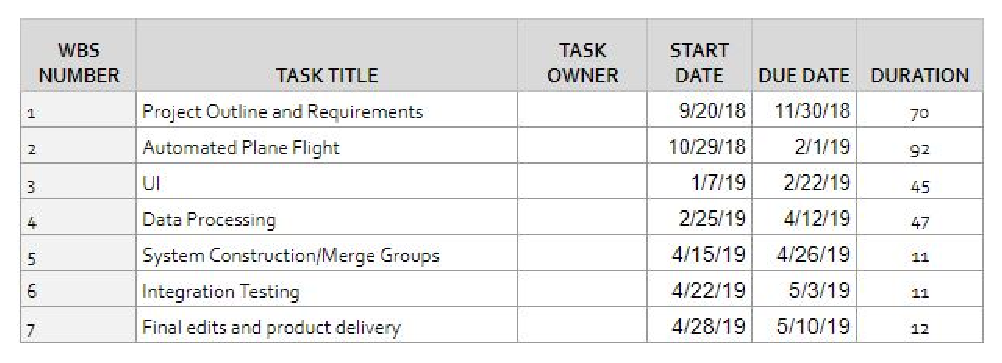
\includegraphics[width=\textwidth]{ganttable.eps}
\newline
\newline
\newline
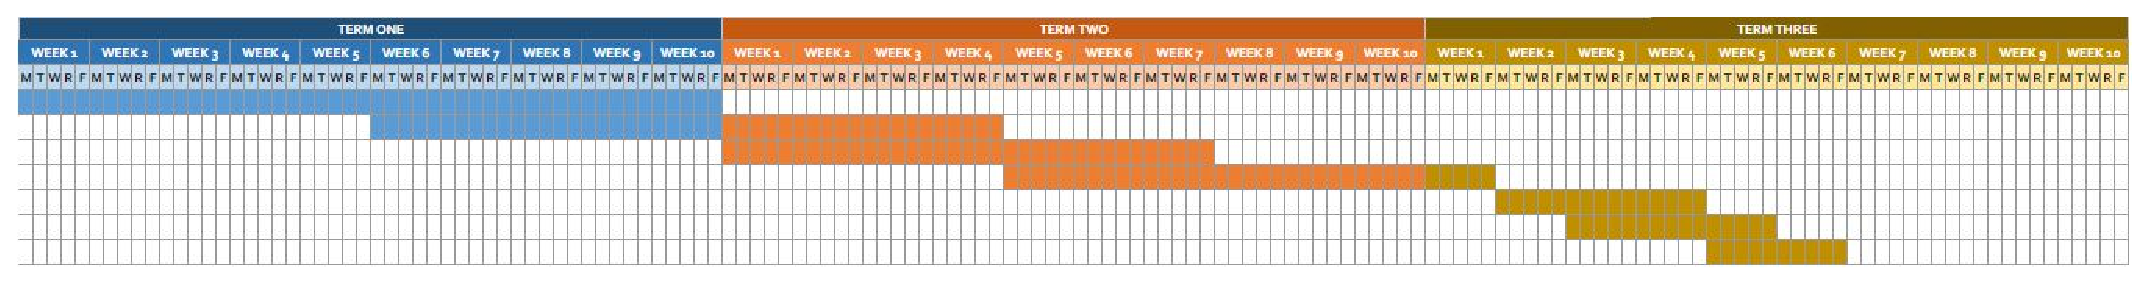
\includegraphics[width=\textwidth]{gantchart.eps}
\end{document}